\chapter{Konzeption}

In diesem Kapitel wird die Konzeption des Gesamtsystems beschrieben. Es wird die Nutzungskontextanalyse beschrieben, welches als Grundlage und Vorbereitung für die anschließende Anforderungsanalyse diente. Die Anforderungsanalyse in welcher, im Rahmen eines Kreativ Workshops, Anwendungsfälle für das zu konzipierende System erarbeitet wurden, wird erläutert. Abschließend wird ein Entwurf der Anwendung beschrieben.

\section{Nutzungskontextanalyse}

% Aktuelle Problemlösungstrategien? Bewertungen auf Online Portalen, Blogs, Interessengruppen, Reklamationen, Technischer Support
Aktuelle Lösungen für die Abgabe von Feedbacks zu Produkten erfolgt oft ohne den Einsatz von Augmented Reality. Diese erfolgen 
oft als Bewertungen in Online Einkaufsportalen, Blog Beiträgen, durch den Austausch in Interessengruppen oder über direkten Kontakt zum Hersteller.

Bei Bewertungen in Onlineportalen, in Blog Beiträgen oder auch bei direktem Kontakt zum Hersteller (z.Bsp. durch E-Mail), haben Kunden die Möglichkeit 
Ihre Feedbacks schriftlich zu beschreiben und mit Bildern oder Videos zu ergänzen. Bei solchen Beschreibungen kommt es jedoch manchmal vor dass 
nicht immer klar hervorgeht zu welcher Stelle oder zu welches Teil am Produkt sich die Beschreibung bezieht. Informationen über die Umgebung in welchem das Produkt 
verwendet wird, geht aus solchen Beschreibungen auch nicht immer hervor. Zudem ist nicht ohne Aufwand möglich direkt zu erkennen an welchen Stellen eines Produktes 
Feedbacks häufen.

Bei Interessengruppen in welchen Nutzer von bestimmten Produkten, sich räumlich zusammentreffen um Erfahrungen auszutauschen wie z.Bsp. zu Hausaltprodukten, Modellflugzeugen, VR Headsets usw., 
haben die Nutzer die Möglichkeit Ihre Ideen genauer zu beschreiben. 
Bei solchen Treffen haben die Nutzer die Möglichkeit mit Bezugnahme auf die Stellen am Produkt und dem Kontext ihrer Umgebung Feedback zum Produkt zu geben. 
Das Problem bei dieser Art der Feedback ist jedoch dessen eingrenzte Reichweite. Zudem werden Inhalte welche in solchen Treffen diskutiert wurden oft nicht ausreichend dokumentiert.  

Auf Basis der im Kapitel \ref{CapterFundamentals} behandelten Grundlagen und der Nutzungskontextanalyse wurde eine abstrakte Skizze des Gesamtsystems (Abbildung \ref{img:sysstem_sketch}) entworfen in welcher, 
Funktionale wie Nicht-Funktionale Anforderungen an das zu konzipierende System dargestellt werden:

\begin{figure}[H]
	\centering
	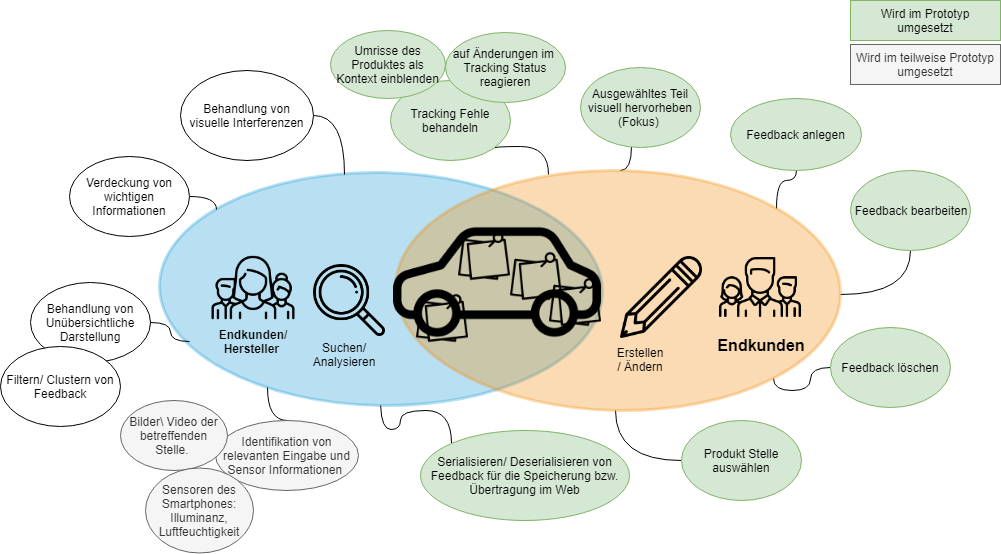
\includegraphics[width=1.0\textwidth]{resources/conception/SystemSkizze.png}
	\caption{Abstrakte Skizze des Gesamtsystems \\Quelle: Eigene Darstellung}
	\label{img:sysstem_sketch}
\end{figure}

Dieses Skizze sollte die Projektidee begreifbarer machen und als grobe Orientierung bei der Anforderungsanalyse dienen.

\section{Anforderungsanalyse}

Als Grundlage für die Anforderungsanalyse wurde ein Kreativ Workshops durchgeführt. Das Ziel dieses Workshops war, die im Kapitel \ref{CapterFundamentals} Abschnitt \ref{UsaEng} beschriebenen Schritte des Usability Engineering Lifecycle nach Nielsen umzusetzen.   

% Vorbereitung
Das Workshop fand, am Fraunhofer IPK in Berlin statt und es nahmen fünf Teilnehmer teil. %Füge noch Informationen zu den Teilenehmer hinzu.

Zur Vorbereitung wurde in einem zuvor für diesen Workshop gebuchten, Besprechungsraum, einzelne Stationen für die am Workshop durchzuführenden Aktivitäten vorbereitet.\footnote{z.Bsp.: Aufstellung eines Pinnwand für die Erstellung eines Affinitätsdiagramms, Abbildungen von Personen für die Erstellung von Personas usw.} Zunächst wurden die Teilnehmer begrüßt und für deren Teilnahme am Workshop bedankt. 
Anschließend wurde der Anlass und der Ablauf des Workshop vorgestellt. 

%Durchführung
Mit Hilfe einer kurzen Präsentation wurde die Projektidee vorgestellt und anhand einer groben Skizze des zu konzipierenden Systems (Abbildung \ref{img:sysstem_sketch}) verdeutlicht. 
Anschließend fand eine Frage- Antwort Runde statt, welches den Teilnehmern die Möglichkeit gab, Rückfragen zu stellen. Somit sollte sichergestellt werden, dass die Projektidee von 
allen Teilnehmer verstanden wurde. 

Nach Vorstellung der Projektidee fand ein Brainstorming statt, dessen Ergebnis in einer Affinitätsdiagramm festgehalten wurden. Dieses diente als Grundlage für die Erstellung von Nutzerprofilen. 
\footnote{Im gewöhnlichen Vorgang für die Erstellung von Affinitätsdiagramme, schreiben Teilnehmer Ideen auf Kärtchen, welche zunächst unsortiert auf ein Pinnwand geheftet werden. 
Anschließend werden die Ideen, gemeinsam besprochen und in Gruppen bzw. Untergruppen sortiert. In dem stattgefundenen Workshop wurden diese Gruppen jedoch im voraus vorgegeben.}

Es sollten Ideen für die Beantwortung folgender Fragen zusammengetragen werden: 

\begin{itemize}
	\item Wer sind die Nutzer (Rolle, Erfahrungsstand,  Lebensstil/ Lebenskontext)?
	\item Was sind aktuelle Problemlösungsstrategien der Nutzer?
	\item Was sind die Ziele der Nutzer?
	\item Wo liegen die Schmerzpunkte mit aktuellen Lösungstretarien?
\end{itemize}\label{list:AffiDiagramm}

Es wurde eine Zeitbegrenzung von 15 Minuten Zeit vorgegeben, innerhalb welcher Ideen zu den, oben genannten Fragen, auf Kärtchen aufgeschrieben wurde.
Folgende Ideen sind dabei entstanden welche im nächsten Schritt als Orientierung für die Erstellung von Personas dienten\footnote{Eine Abbildung des entstandenen Affinitätsdiagramm befindet sich im Anhang [Referenz darauf]}: 

\vspace{2mm}
\textit{Wer sind die Nutzer:} 
Technik Nerd, Produkt Entwickler, Werbeagentur, Unzufriedene, Unerfahrene, Gewerbliche Nutzer/ Laborpersonal, Endkunde, Qualitätsprüfung eines Produkts (Vorgesetzter), Lagerpersonal

\vspace{2mm}
\textit{Aktuelle Problemlösungsstrategien:} 
Email, Chat, Web-Portale, Telefonsupport, Vergleich von Käuferbewertungen

\vspace{2mm}
\textit{Ziele der Nutzer: } 
Nächstes Produkt sollte besser sein, Eigenes Design, Fehleranfälligkeit beseitigen, Informationen vor dem Kauf, Hilfreiche Bewertungen finden und verstehen, Ersatzteile beschaffen, Lösungen aus dem Nutzerkreis bereitstellen, Infos in Form: Kurzer Beschreibungen/ Kontakt Informationen des Verantwortlichen, Anleitungen, Reklamation Technischer Dokumentationen (Montageanleitung)

\vspace{2mm}
\textit{Wo liegen die Schmerzpunkte: } 
Komplizierte Beschreibung der Umgebung/ Use-Case, Zustand der Bearbeitung unbekannt, Fehlerbehebung meines Produktes, Produkt wird nicht wie vorgesehen (geplant) genutzt und funktioniert daher nicht richtig (Vorstellung eines möglichen neuen Anwendungsfalles), Lange Wartezeiten auf Antwort, Bessere Kommunikation zwischen Abteilungen

\textbf{Personas}:
%Durchführung %Aufbau / Einleitung / Affinitätsdiagram / Personas / Szenarien
Im nächsten Schritt wurden auf Grundlage der im  Affinitätsdiagramm festgehaltenen Stichpunkte, Personas erstellt. Diese repräsentieren, stellvertretend die Ziele der 
Nutzer des zu konzipierenden Systems.

Es wurden Bilder von Personen unterschiedlicher Alter und Geschlecht auf dem Boden ausgelegt. Die Bilder zeigten die Personen in jeweils unterschiedlichen Situationen, 
sodass möglichst individuelle Eigenschaften ausgemacht werden konnten. Es fand eine kurze Diskussion statt indem, Abbildungen von Personen ausgewählt wurden welche, realistische 
Nutzer für das zu konzipierende System darstellen. Anschließend wurden den Personas fiktive Namen gegeben und die Begriffe aus dem Affinitätsdiagramm in gemeinsamer Abstimmung den 
einzelnen Personen zugeordnet. 

Auf diese weise wurde in Anlehnung an das in \cite[S.~57]{MichaelRichter2016} vorgestellte Beispiel, fünf unterschiedliche Personas erstellt (Tabelle \ref{tab:personas}, Eine vollständige Beschreibung der Personas befindet sich im Anhang \ref{anhangA}). Die Personas, Felix, Timo und Svenja sind für die Implementierung des Prototypen besonders bedeutsam. Diese Personas werden das System nutzen um Feedbacks zu erstellen, 
zu bearbeiten und zu löschen. Die Personas Magitta und Flo dienen dazu um ein Verständnis für das zu konzipierende Gesamtsystem aufzubauen in welchem sich der Prototyp einfügen soll. Diese werden vorwiegend die Artefakte 
welche durch das System entstehen nutzen. 

\begin{table}[htbp]
	\caption{Zusammenfassung der Personas}
		\begin{tabular}{|l|l|l|}
			\hline
			 \textbf{Name} & \textbf{Rolle}& \textbf{Ziele und Bedürfnisse}\\
			\hline
			\textbf{Timo} &  Produktentwickler & \makecell[l]{*Oft sind komplizierte Anwendungsfälle schwer zu beschreiben.\\ *Produktbezogene Beschreibungen bei welchen Bezug zu \\spezifischen Stellen  am Produkt\\ genommen werden muss\\ oft von anderen nicht verstanden.} \\
			\hline
			\textbf{Svenja} & Auszubildende & * \makecell[l]{Möchte dass es besonders einfach und unkompliziert benutzbar ist.}\\
			\hline
			\textbf{Felix} & Zahnarzt &  \makecell[l]{* Möchte dass seine Laborgeräte \\einwandfrei funktionieren.\\ * Möchte bei technischen Problemen schnelle\\ * Rückmeldung vom Hersteller. \\Qualität der Produkte\\ haben einen Einfluss auf sein Betrieb.} \\
			\hline
			\textbf{Magitta} & Produktmanagerin & \makecell[l]{* Möchte die Produkte\\ ihres Unternehmens zu verbessern.\\ * Wo liegen die Schwächen? Wo die Stärken?\\* Wie werden die Produkte von \\den Kunden wahrgenommen?}\\
			\hline
			\textbf{Flo} & Daten Analyst & \makecell[l]{* Möchte aus Daten Wissen generieren.\\ * Möchte über eine Schnittstelle präzise\\ Kundenfeedbacks zu Produkten erheben\\ um aus diesen Erkenntnisse zu generieren}\\ 
			\hline
		\end{tabular}
	\label{tab:personas}
\end{table}

\textbf{Szenarien}:

Basierend auf den entworfenen Personas, wurden im nächsten Schritt Ist-Szenarien beschrieben (Siehe Anhang: \ref{anhangA} Abschnitt Ist-Szenarien). Mit diesen wurden aktuelle Problemlösungsstrategien der Personas Timo, Felix und Svenja im jeweiligen Anwendungskontext beschrieben. Dabei wurden besonders die Schmerzpunkte der aktuellen Lösungstretarien betont. Die Ist-Szenarien wurden hinsichtlich mögliche Verbesserungen mit einer neuen Lösung analysiert und im weiteren Schritt wurden Soll-Szenarien entwickelt (Siehe Anhang \ref{anhangA} Abschnitt Soll-Szenarien). 

Die Soll-Szenarien beschreiben, in welchem Kontext sowie unter welchen Bedingungen die Anwendung verwendet wird um die Aufgabe, ein Feedback an einem physischen Produkt abzugeben. 
Die beschriebenen Soll-Szenarien beinhalten Beschreibungen für Funktionen welche nicht im Prototypen enthalten sein werden. Diese dienen dazu um ein Verständnis dafür aufzubauen zu können, wie sich der Prototyp in ein Gesamtsystem mit diesen Funktionen einfügen wird. 

Funktionen welche in den Ist-Szenarien beschrieben werden jedoch nicht Teil des Prototypen sein werden: 

\begin{itemize}
\item{Anmeldevorgang} 
\item{Produktauswahl} 
\item{Feedbacks von anderen Nutzern auf dem Produkt sehen}
\item{Versand von Informationen an den Hersteller}
\end{itemize}

%Svenja. Praktisch, schnell. 
%Felix Vorgang zum Auswählen eines teils + Wunsch äußern dass Rückmeldung vom Hersteller erwünscht ist.
%Timo Kategorien zum Auswählen

\textbf{User Stories}:

Auf Grundlage der Soll-Szenarien, wurden im nächsten Schritt User Stories beschrieben welche im Prototypen implementiert werden: 

%\begin{center}
	\begin{table}[htbp]
	\caption{User Stories}
	\resizebox{\textwidth}{!}{
	\begin{tabular}{ | c | c | c |c |c |}
		\hline
		\thead{Nr.} & \thead{Als} & \thead{abgeleitet \\ aus \\ Persona} &	\thead{möchte ich} & \thead{damit} \\
		\hline
		10 &  \makecell{Endkunde} & \makecell{Timo} & \makecell{neue Anwendungsfälle \\direkt am Produktteil\\ beschreiben können} &  \makecell{ich bei meiner Beschreibung\\ implizit ein Bezug\\
			zu einer bestimmten\\ Stelle am Produkt\\ herstellen kann.} \\
		\hline
		20 &  \makecell{Endkunde} & \makecell{Timo} & \makecell{Ergänzende Anleitungen direkt\\ am  Produktteil\\ oder Stellen ansehen können} &  \makecell{ich mir ergänzende Bemerkungen \\und Anleitungen
			direkt an der \\ betreffenden Stelle ansehen kann.
} \\
		\hline
		30 &  \makecell{Endkunde} & \makecell{Timo} & \makecell{Anleitungen zu spezifischen\\ Stellen am Produkt \\beschreiben können} &  \makecell{mir die Bezugnahme zu der\\ betreffenden Stelle
			am Produkt\\ erleichtert wird und meine \\Anleitungen
			verständlicher \\für andere werden.} \\
		\hline
		31 &  \makecell{Endkunde)}  & \makecell{Svenja, \\ Timo, \\ Felix} & \makecell{ein bestimmtes Teil an einem\\
			physischen Produkt auswählen\\
			können
} &  \makecell{ich bezugnehmend auf das ausgewählte\\ Teil
			Aktionen ausführen kann.\\ (z. B.: eine
			Rückmeldung abgeben)}\\
		\hline
		32 &  \makecell{Endkunde}  & \makecell{Svenja, \\ Timo, \\ Felix} & \makecell{eine von mir abgegebenes\\
			Feedback auswählen können,} &  \makecell{damit ich dieses Feedback oder den\\
			löschen kann}\\
		\hline
		33 &  \makecell{Endkunde}  & \makecell{Svenja, \\ Timo, \\ Felix} & \makecell{die Beschreibung auf einer von mir\\
			abgegebenes Feedback verändern\\
			können} &  \makecell{ich eine Nachträgliche Korrektur oder Ergänzung\\
			vornehmen zu kann.
}\\
		\hline
		34 &  \makecell{Endkunde}  & \makecell{Svenja, \\ Timo, \\ Felix} & \makecell{den Bezugspunkt (Produktteil oder\\
			bestimmte Stelle auf einem\\
			Produktteil) auf die, ein von mir\\
			erstelltes Feedback sich bezieht\\
			ändern können
} &  \makecell{ich eine Nachträgliche Korrektur oder Ergänzung\\
			vornehmen zu kann.
}\\
		\hline
		35 &  \makecell{Endkunde}  & \makecell{Svenja, \\ Timo, \\ Felix} & \makecell{ein von mir erstelltes Feedback\\
			löschen können} &  \makecell{ich eine obsolete, redundante oder versehentlich\\
			erstellte Rückmeldung wieder entfernen kann.}\\
		\hline
		40 &  \makecell{Endkunde}  & \makecell{Svenja} & \makecell{schnell und unkompliziert\\
			Feedbacks zu Teile od. Stellen am Produkt\\
			abgeben können.} &  \makecell{ich auch Feedbacks beiläufig abgeben kann.}\\
		\hline	
		50 &  \makecell{Endkunde}  & \makecell{Svenja, \\ Timo, \\ Felix} & \makecell{Bewertungen zu ein\\
			Produkt, an der Betreffenden Stelle am\\ Produkt ansehen können} &  \makecell{ich mich vor dem Kauf eines Produktes genauer\\
			erkundigen kann, und mir vor allem, die für mich
			wichtigen stellen am \\Produkt besser beurteilen
			kann
}\\
		\hline	
		60 &  \makecell{Endkunde}  & \makecell{Svenja, \\ Timo, \\ Felix} & \makecell{Kontaktinformationen zu\\
			Verantwortlichen Personen sehen\\
			können.} &  \makecell{ich direkt Kontakt zu dieser Person aufnehmen\\
			kann.}\\
		\hline	
		70 &  \makecell{Geschäftskunde\\(gewerblich\\nutzender\\Endkunde)}  & \makecell{Felix} & \makecell{möchte ich den Wunsch äußern\\
			können, dass der Hersteller über mein\\
			Feedback informiert wird} &  \makecell{ich sichergehen kann dass mein Feedback\\
			zeitnah vom Hersteller wahrgenommen wird}\\
		\hline	
		80 &  \makecell{Geschäftskunde\\(gewerblich\\nutzender\\Endkunde)}  & \makecell{Felix} & \makecell{bei Abgabe eines Feedback,\\ den
			Einfluss auf mein Geschäft\\ oder Anwendungsfall \\
			beschreiben können} &  \makecell{ich dem Hersteller des Produktes\\ ein besseres Verständnis über den Ausmaß ermöglichen\\ kann und dieser den im Feedback\\ entsprechend beurteilen und priorisieren kann }\\
		\hline	
\end{tabular}}
	\label{tab:userstories}	
\end{table}
%\end{center}

\section{Entwurf}

Im folgenden Abschnitt wird der erste Entwurf des zu entwickelnden Prototypen beschrieben. Es wird zunächst ein Papierprototyp vorgestellt welches ein Entwurf der Benutzeroberfläche darstellt. 
Anschließend werden die einzelnen Module vorgestellt welche das System besitzen wird. Anschließend werden die durch das System zu speichernden Daten in Form einer Entitätentyp festgelegt und dargestellt
sowie die Klassendiagramme für den digitalen Prototypen entworfen.  

\subsection{Low-Fidelity-Prototyp}

Die in der Anforderungsanalyse erstellten Soll-Szenarien sowie die festgelegten User Stories wurden zur Orientierung für die Gestaltung des Papierprototypen verwendet
Folgend werden die einzelnen Ansichten des entwickelten Papierprototypen vorgestellt und erläutert: 
%Es wurden Techniken 

Auf Abbildung \ref{img:pp_start} ist das Startbildschirm der Anwendung zu sehen. Auf diesem Bildschirm gelangt der Nutzer sobald die Anwendung gestartet wurde. 
In dieser Ansicht wird auf der Mitte des Bildschirms ein Text eingeblendet, welches den Nutzer dazu auffordert, die Kamera auf das Produkt\footnote{Das Wort ``Product`` wird an dieser Stelle in der Annahme verwendet dass für das Tracking ein CAD Modell des physischen Produktes verwendet wird. Dies kann sich je nach verwendeter Tracking Methode ändern. } zu richten. Dieser Text 
wird eingeblendet, damit die Registrierung des Produktes stattfinden kann. 

Auf der linken oberen Ecke des Bildschirms befinden sich zwei Buttons mit den Aufschriften ``My Feedbacks`` und ``New Feedbacks``. Durch das klicken auf das Button ``My Feedbacks`` gelangt der Nutzer in 
das auf Abbildung \ref{fig:pplist} vorstellte Ansicht in welchem der Nutzer die Möglichkeit hat die von ihm erstellen Feedbacks zu bearbeiten oder zu löschen. Klickt der Nutzer auf das Button mit der Aufschrift 
``New Feedbacks`` gelangt er in das auf Abbildung \ref{img:ppcreate} dargestellte Ansicht. In dieser ist die Anwendung in deinem Modus in welcher Produktteile für die Erstellung neuer Feedbacks ausgewählt werden können. 

\begin{figure}[H]
	\centering
	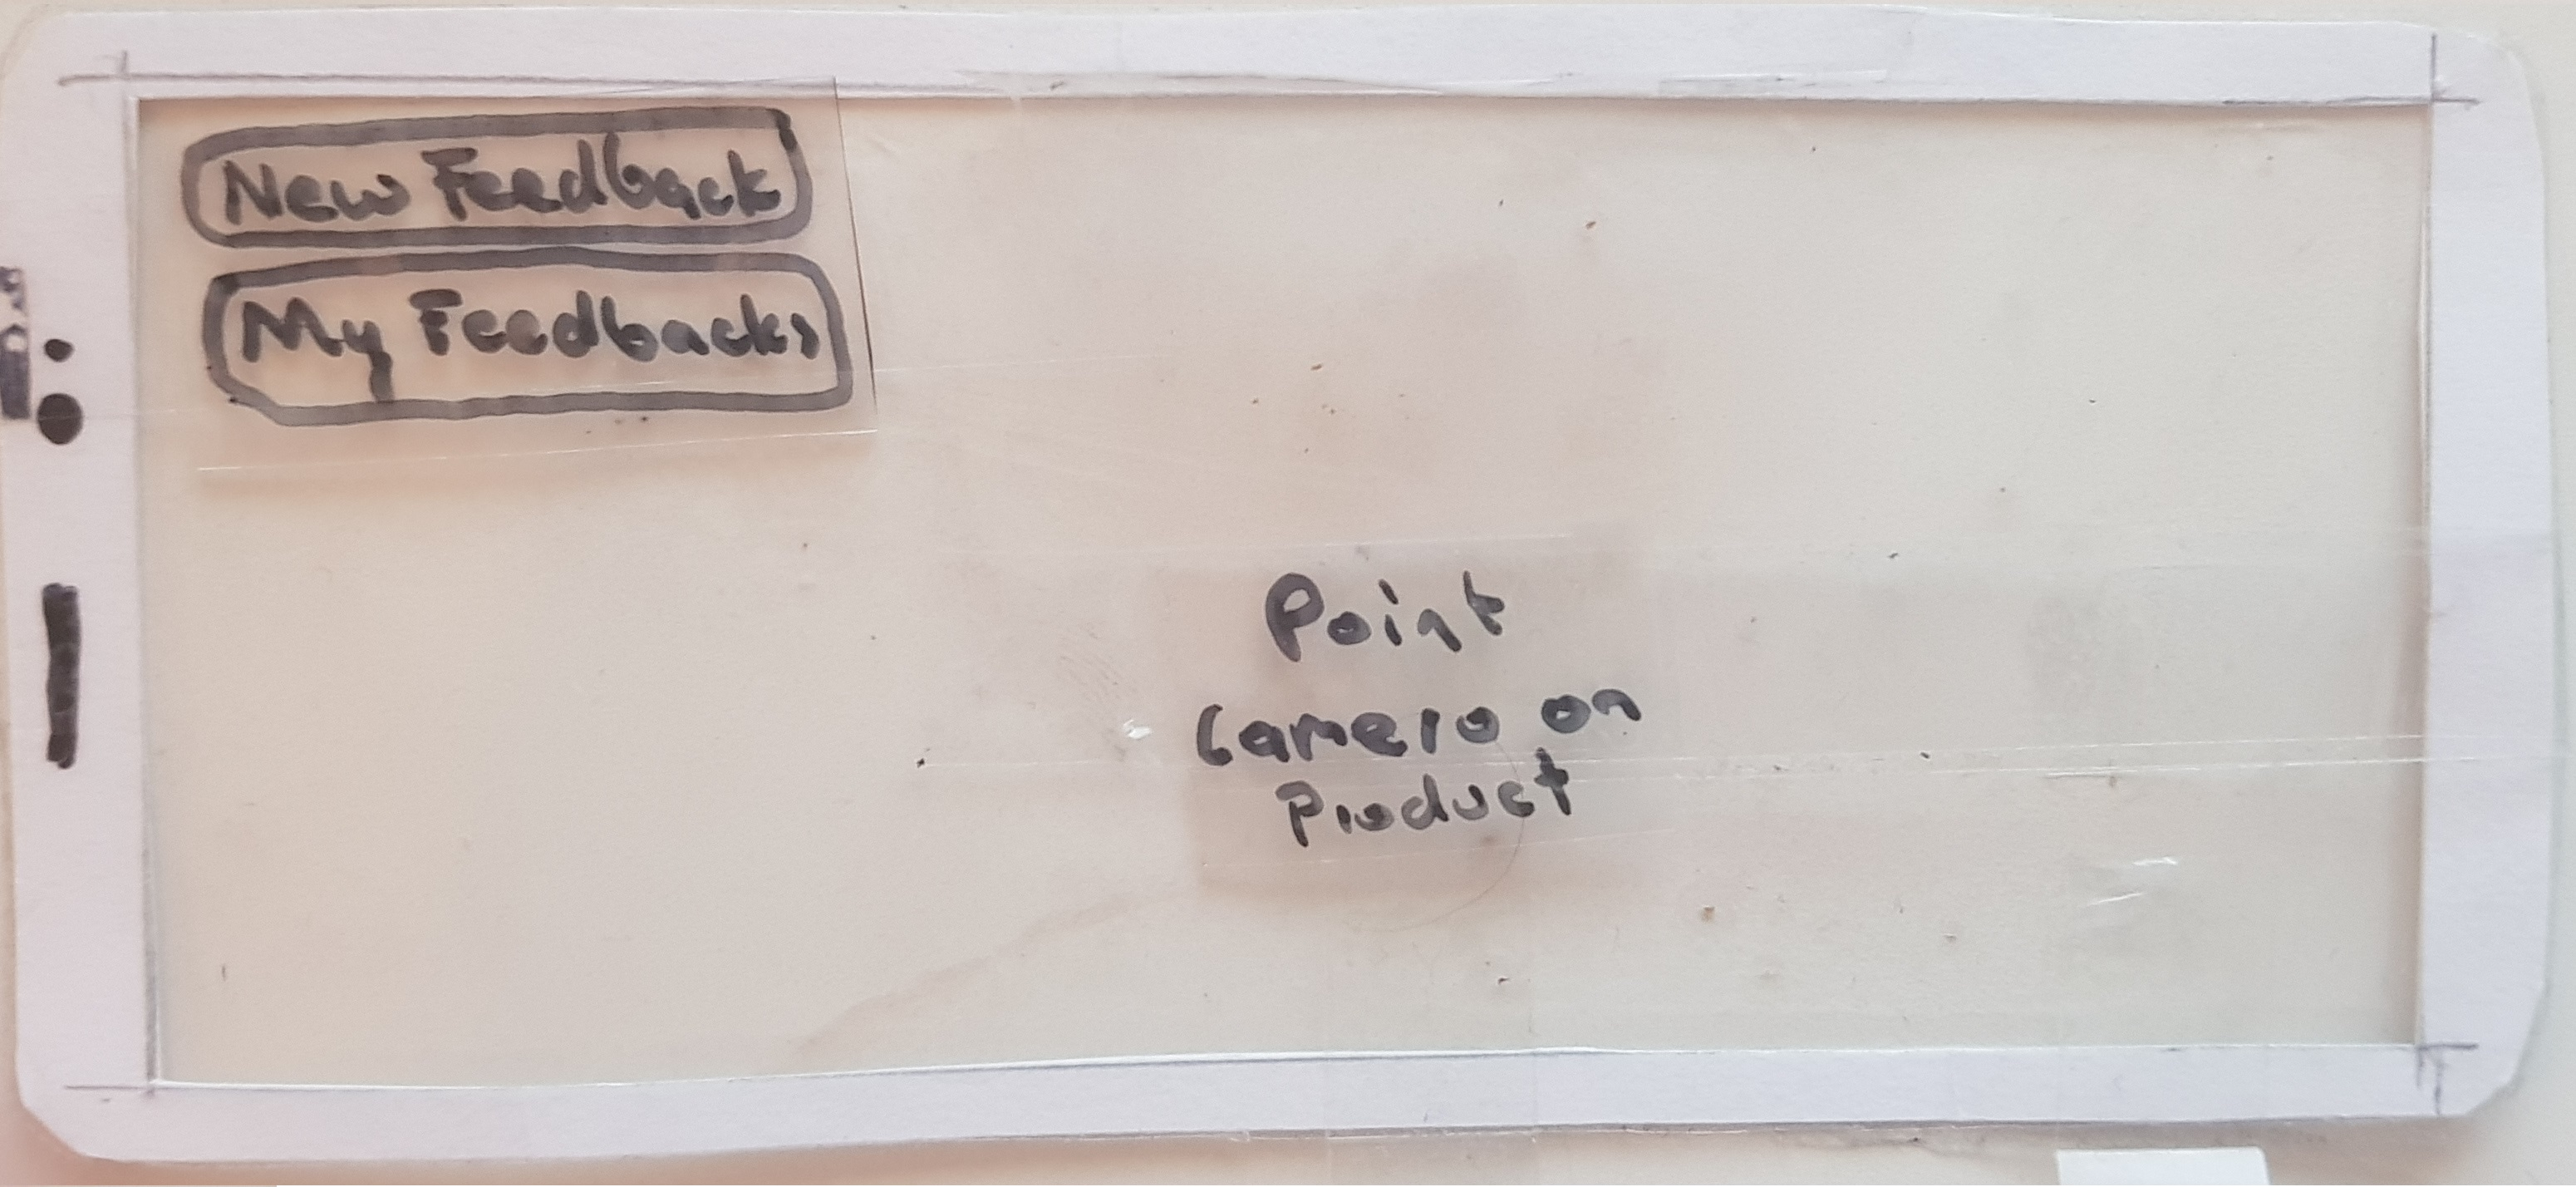
\includegraphics[width=.7\textwidth]{resources/conception/lowfi_startbildschirm.jpg}
	\caption{Papierprototyp - Startbildschirm  \\Quelle: Eigene Darstellung}
	\label{img:pp_start}
\end{figure}

\begin{figure}[H]
	\centering
	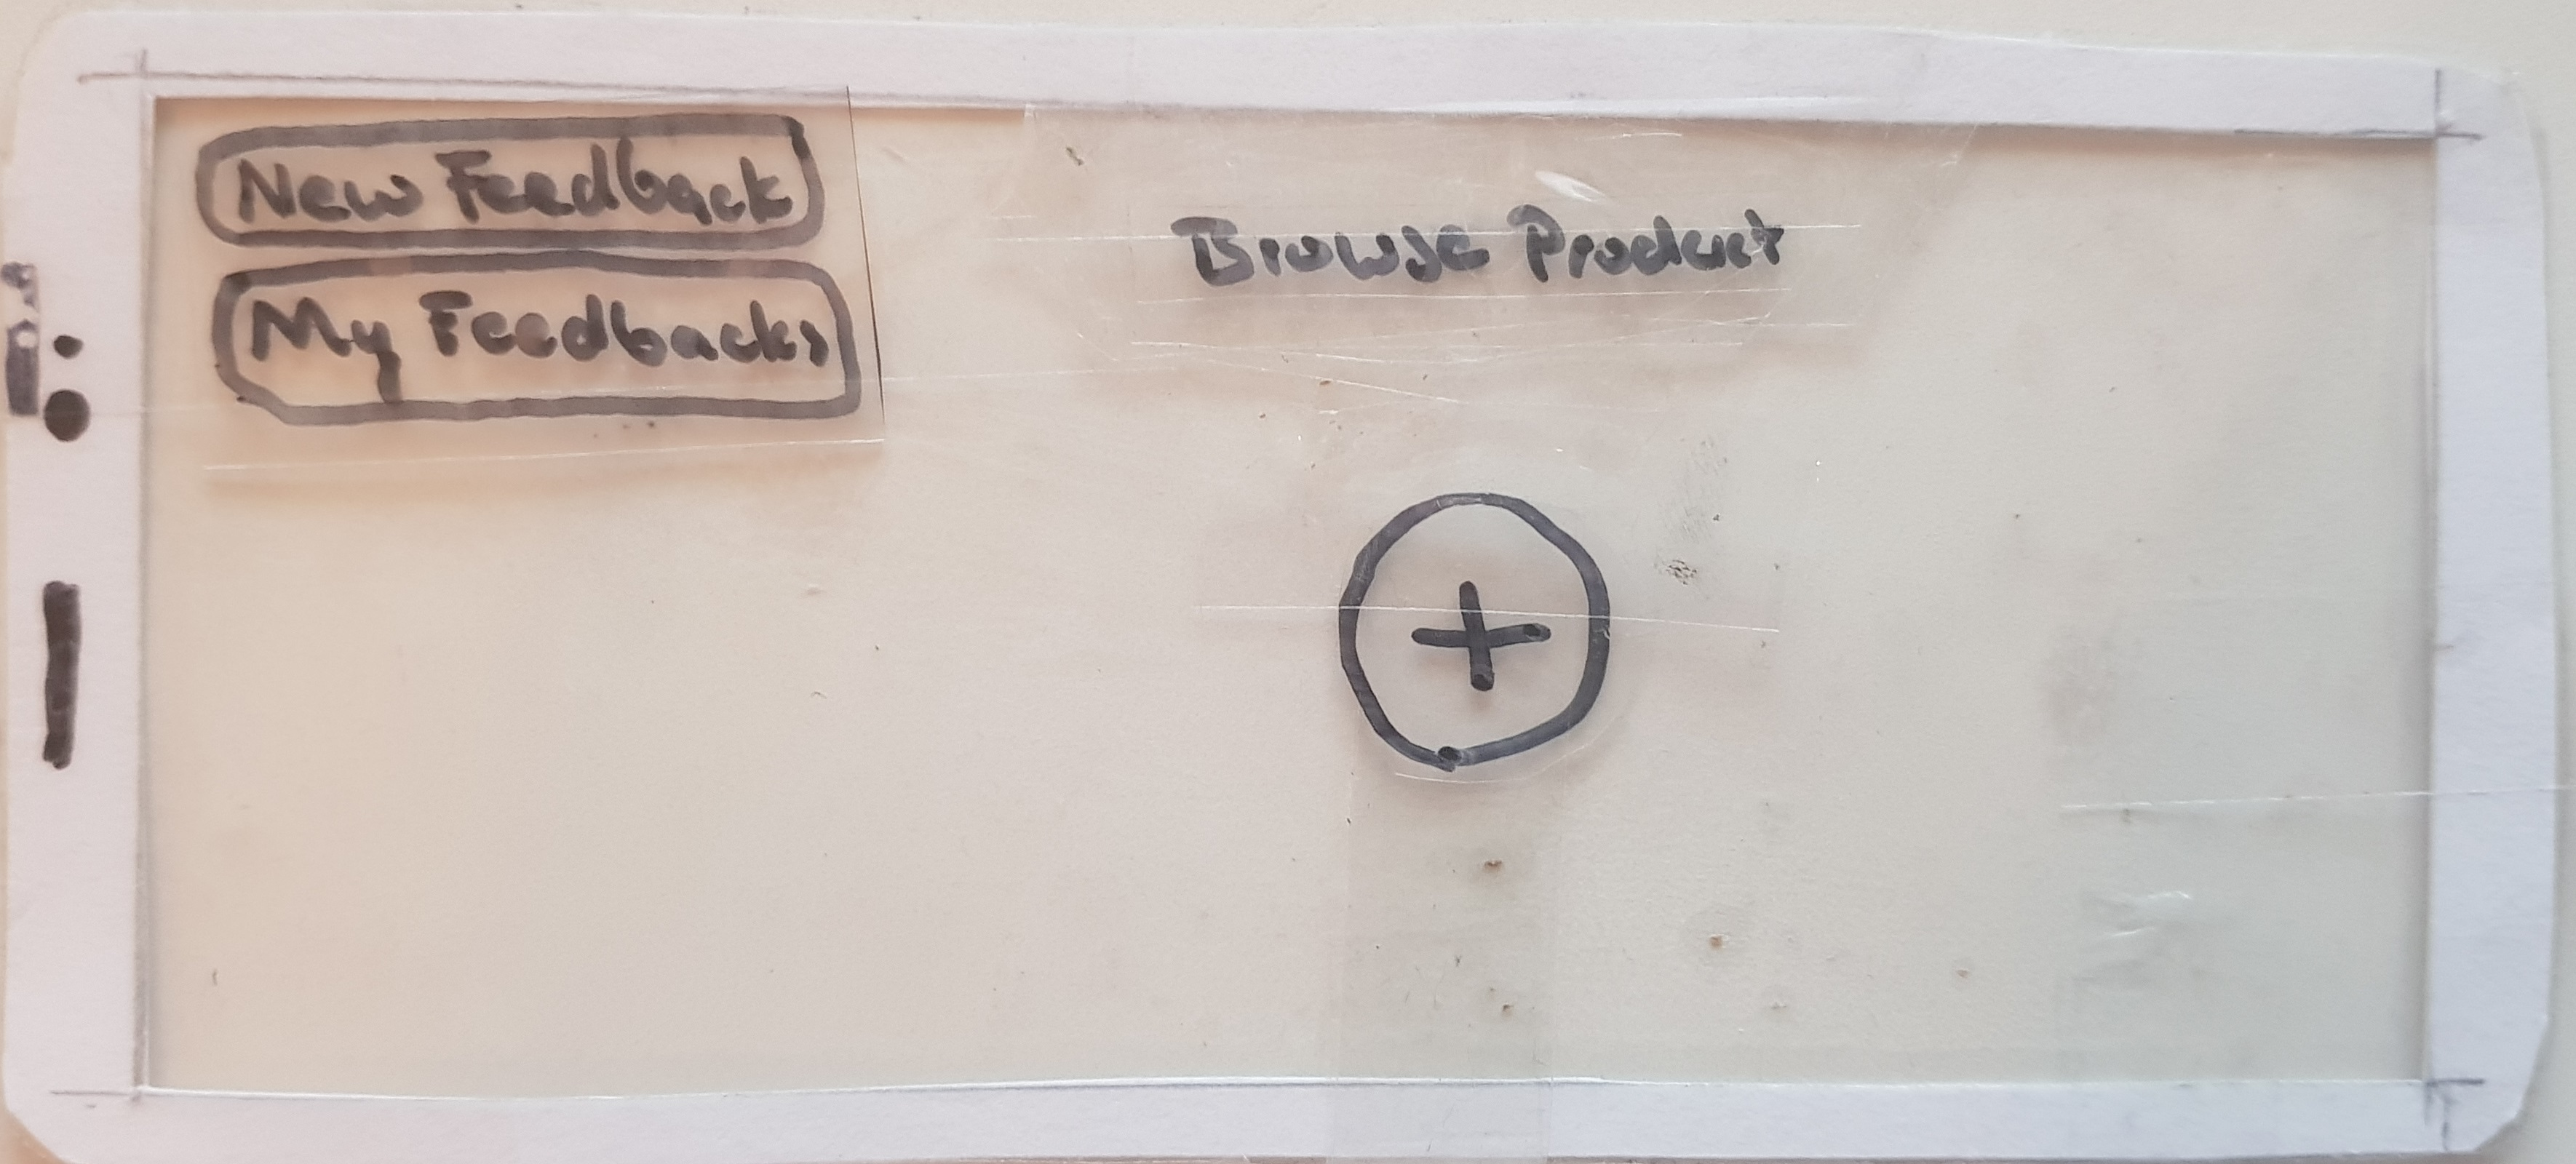
\includegraphics[width=.7\textwidth]{resources/conception/lowfi_browseOnProduct.jpg}
	\caption{Papierprototyp - Ansicht zum Suchen und Finden von Feedbacks auf dem Produkt. \\Quelle: Eigene Darstellung}
	\label{img:sysstem_sketch}
\end{figure}

\begin{figure}[H]
	\centering
	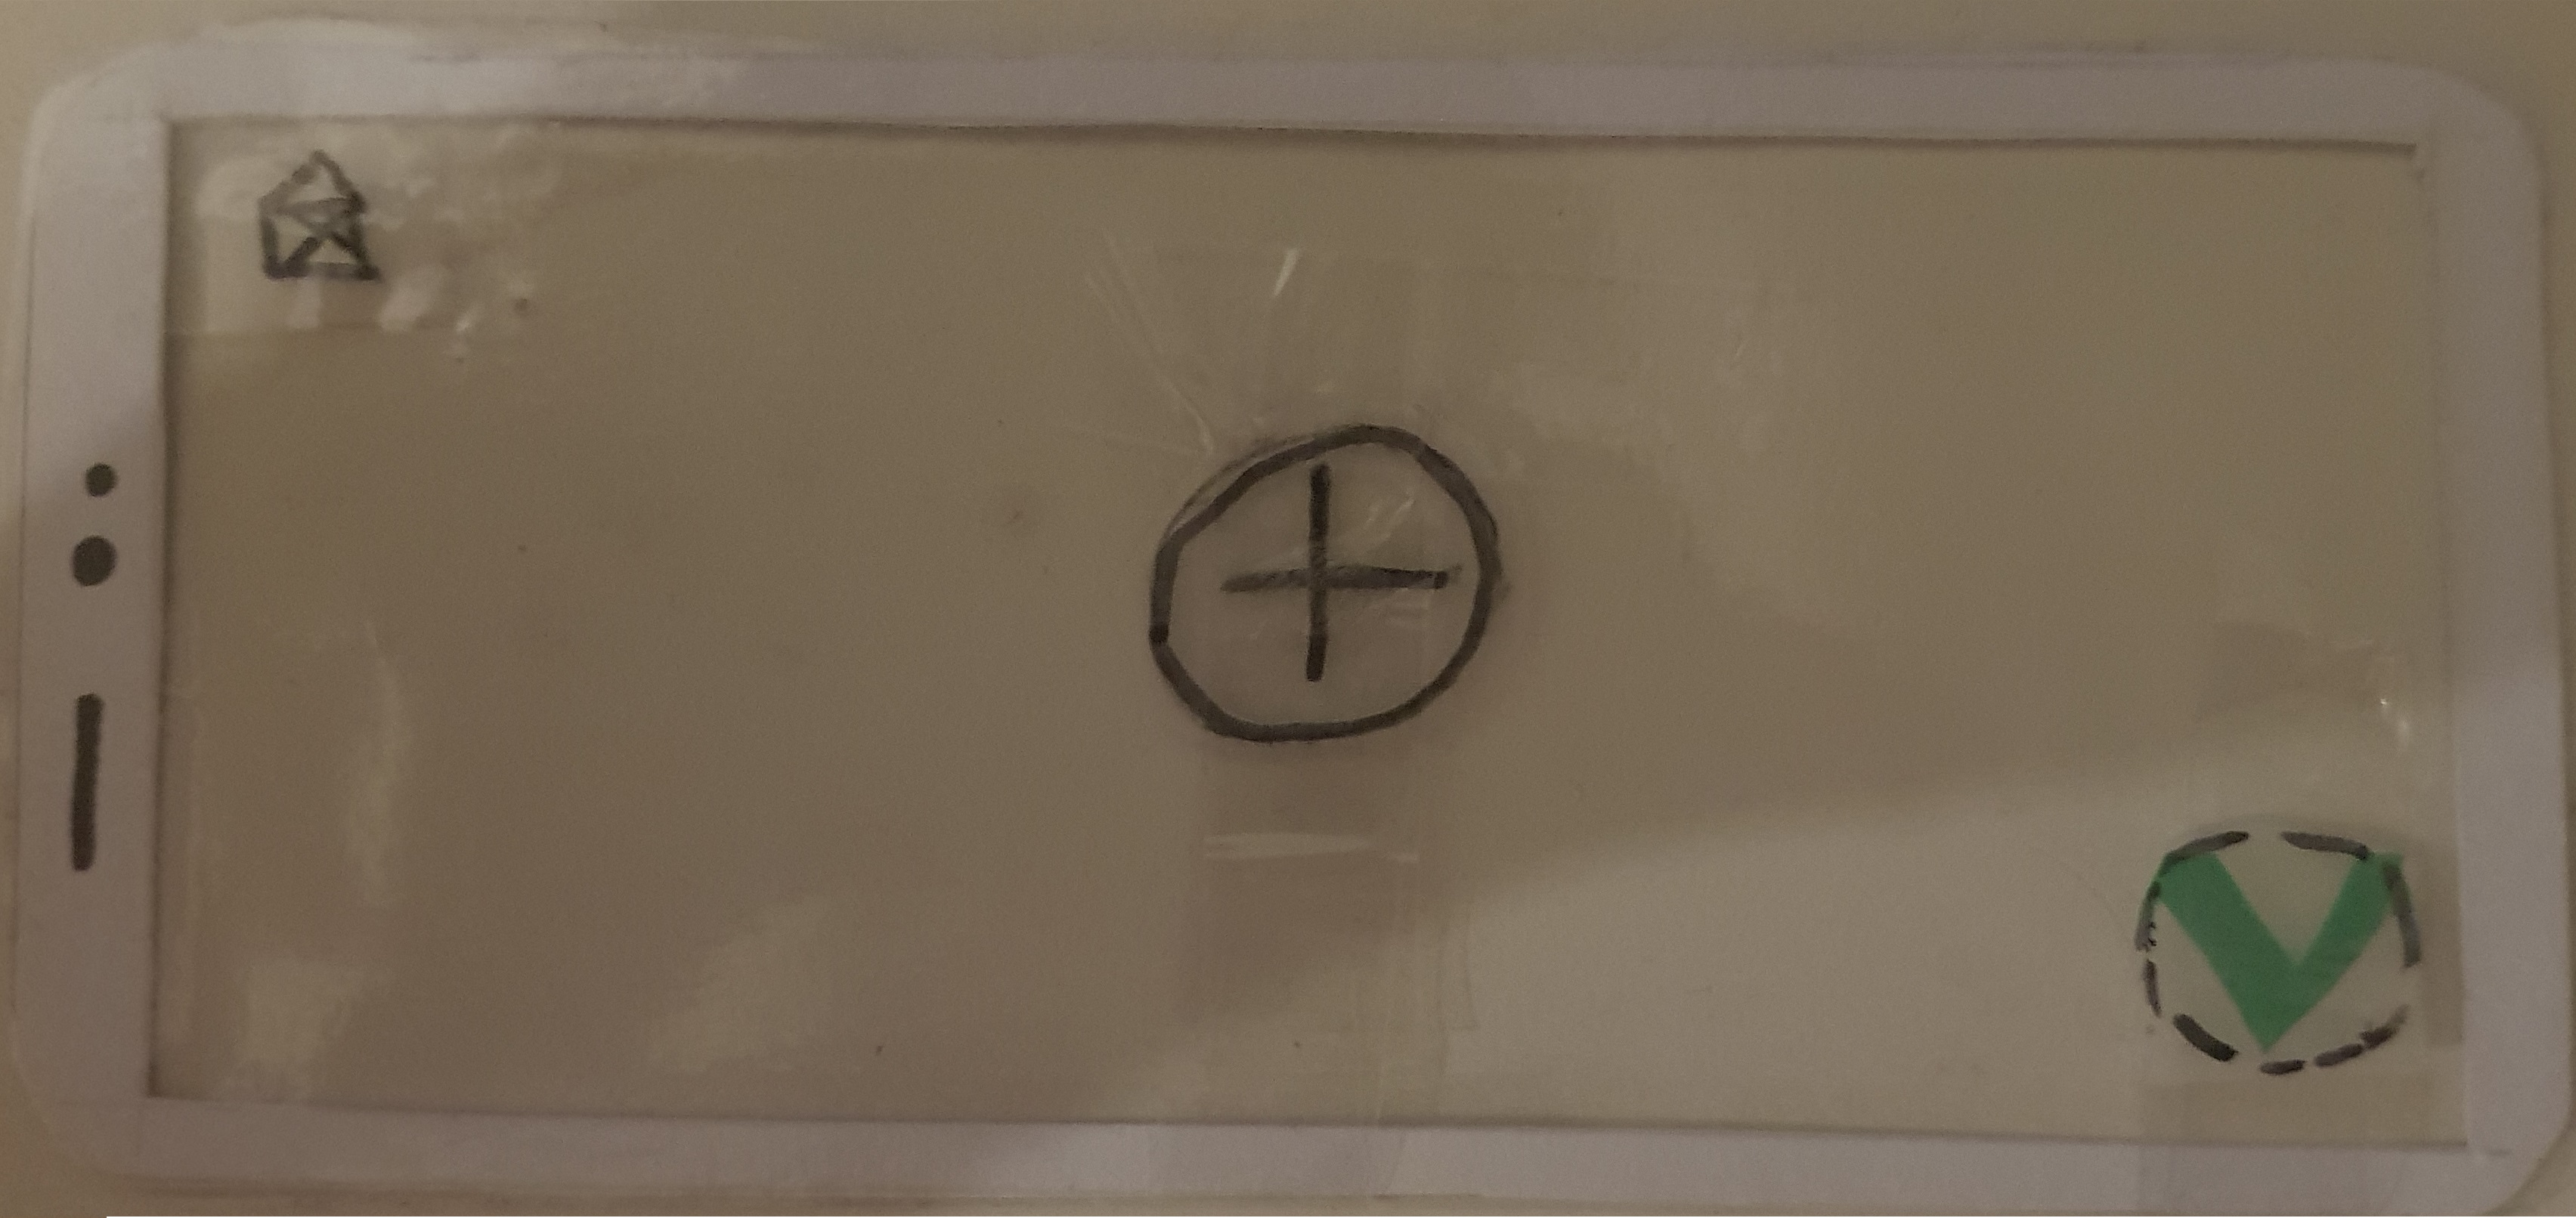
\includegraphics[width=.7\textwidth]{resources/conception/lowfi_create.jpg}
	\caption{Papierprototyp - Auswahl von Produktteil für die Erstellung eines neuen Feedback \\Quelle: Eigene Darstellung}
	\label{img:ppcreate}
\end{figure}

\begin{figure}[H]
	\centering
	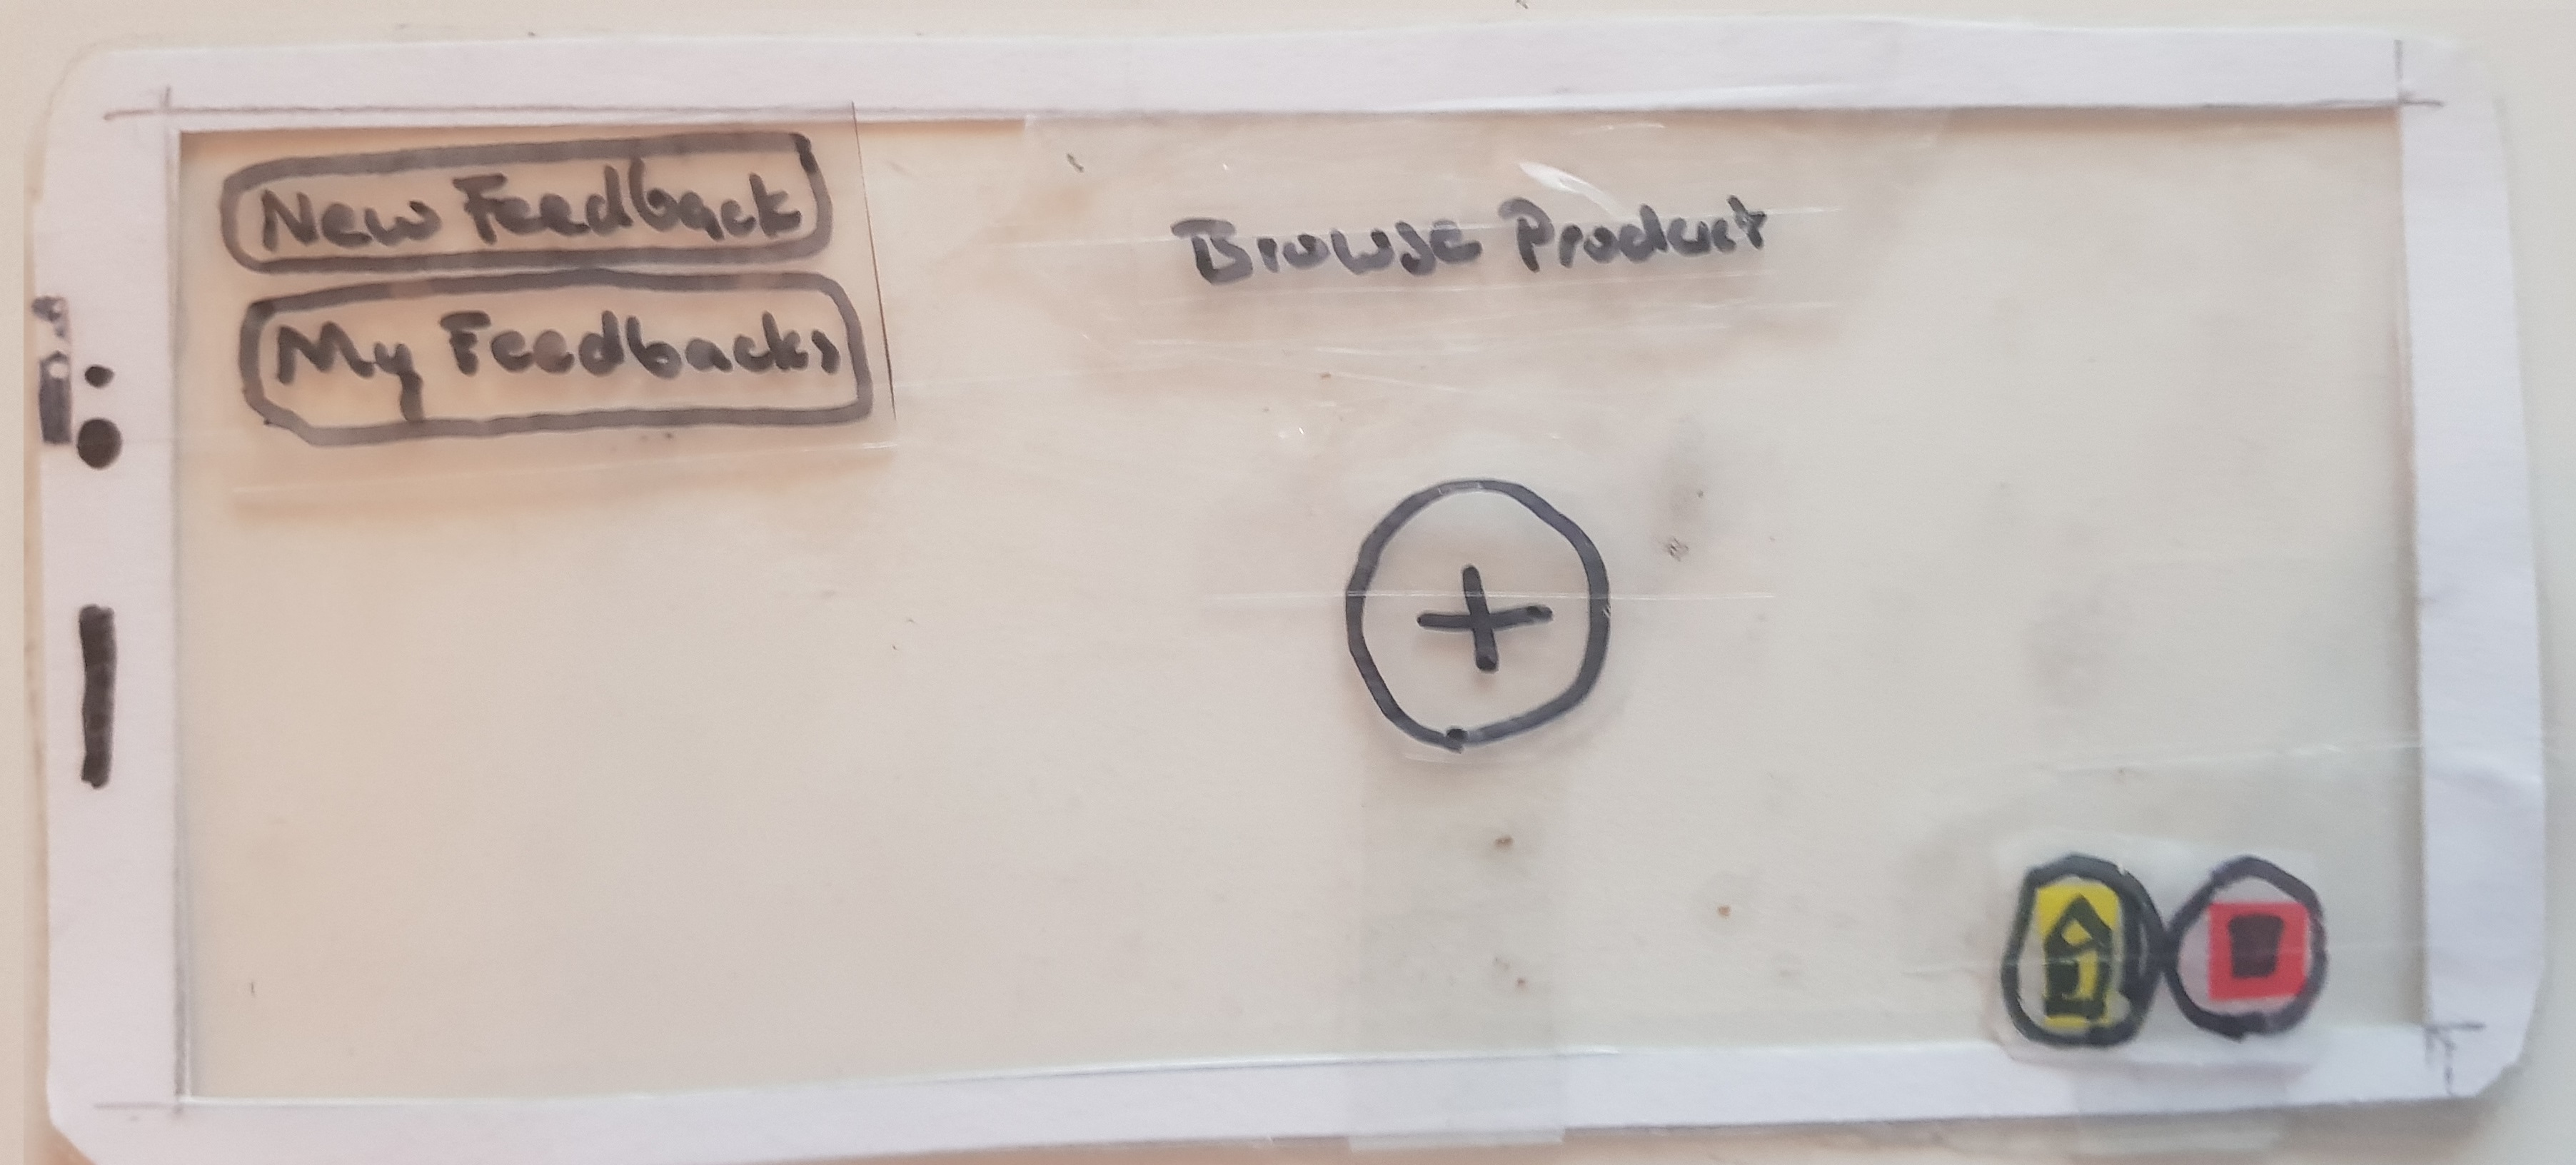
\includegraphics[width=.7\textwidth]{resources/conception/lowfi_edit_delete.jpg}
	\caption{Papierprototyp - Auswahl von Feedback auf dem Produkt für die Bearbeitung bzw. Löschung. \\Quelle: Eigene Darstellung}
	\label{img:sysstem_sketch}
\end{figure}

\autoref{tab:example} 
\begin{figure}[H]
	\label{tab:example}
	\centering
	\begin{minipage}{.5\textwidth}
		\centering
		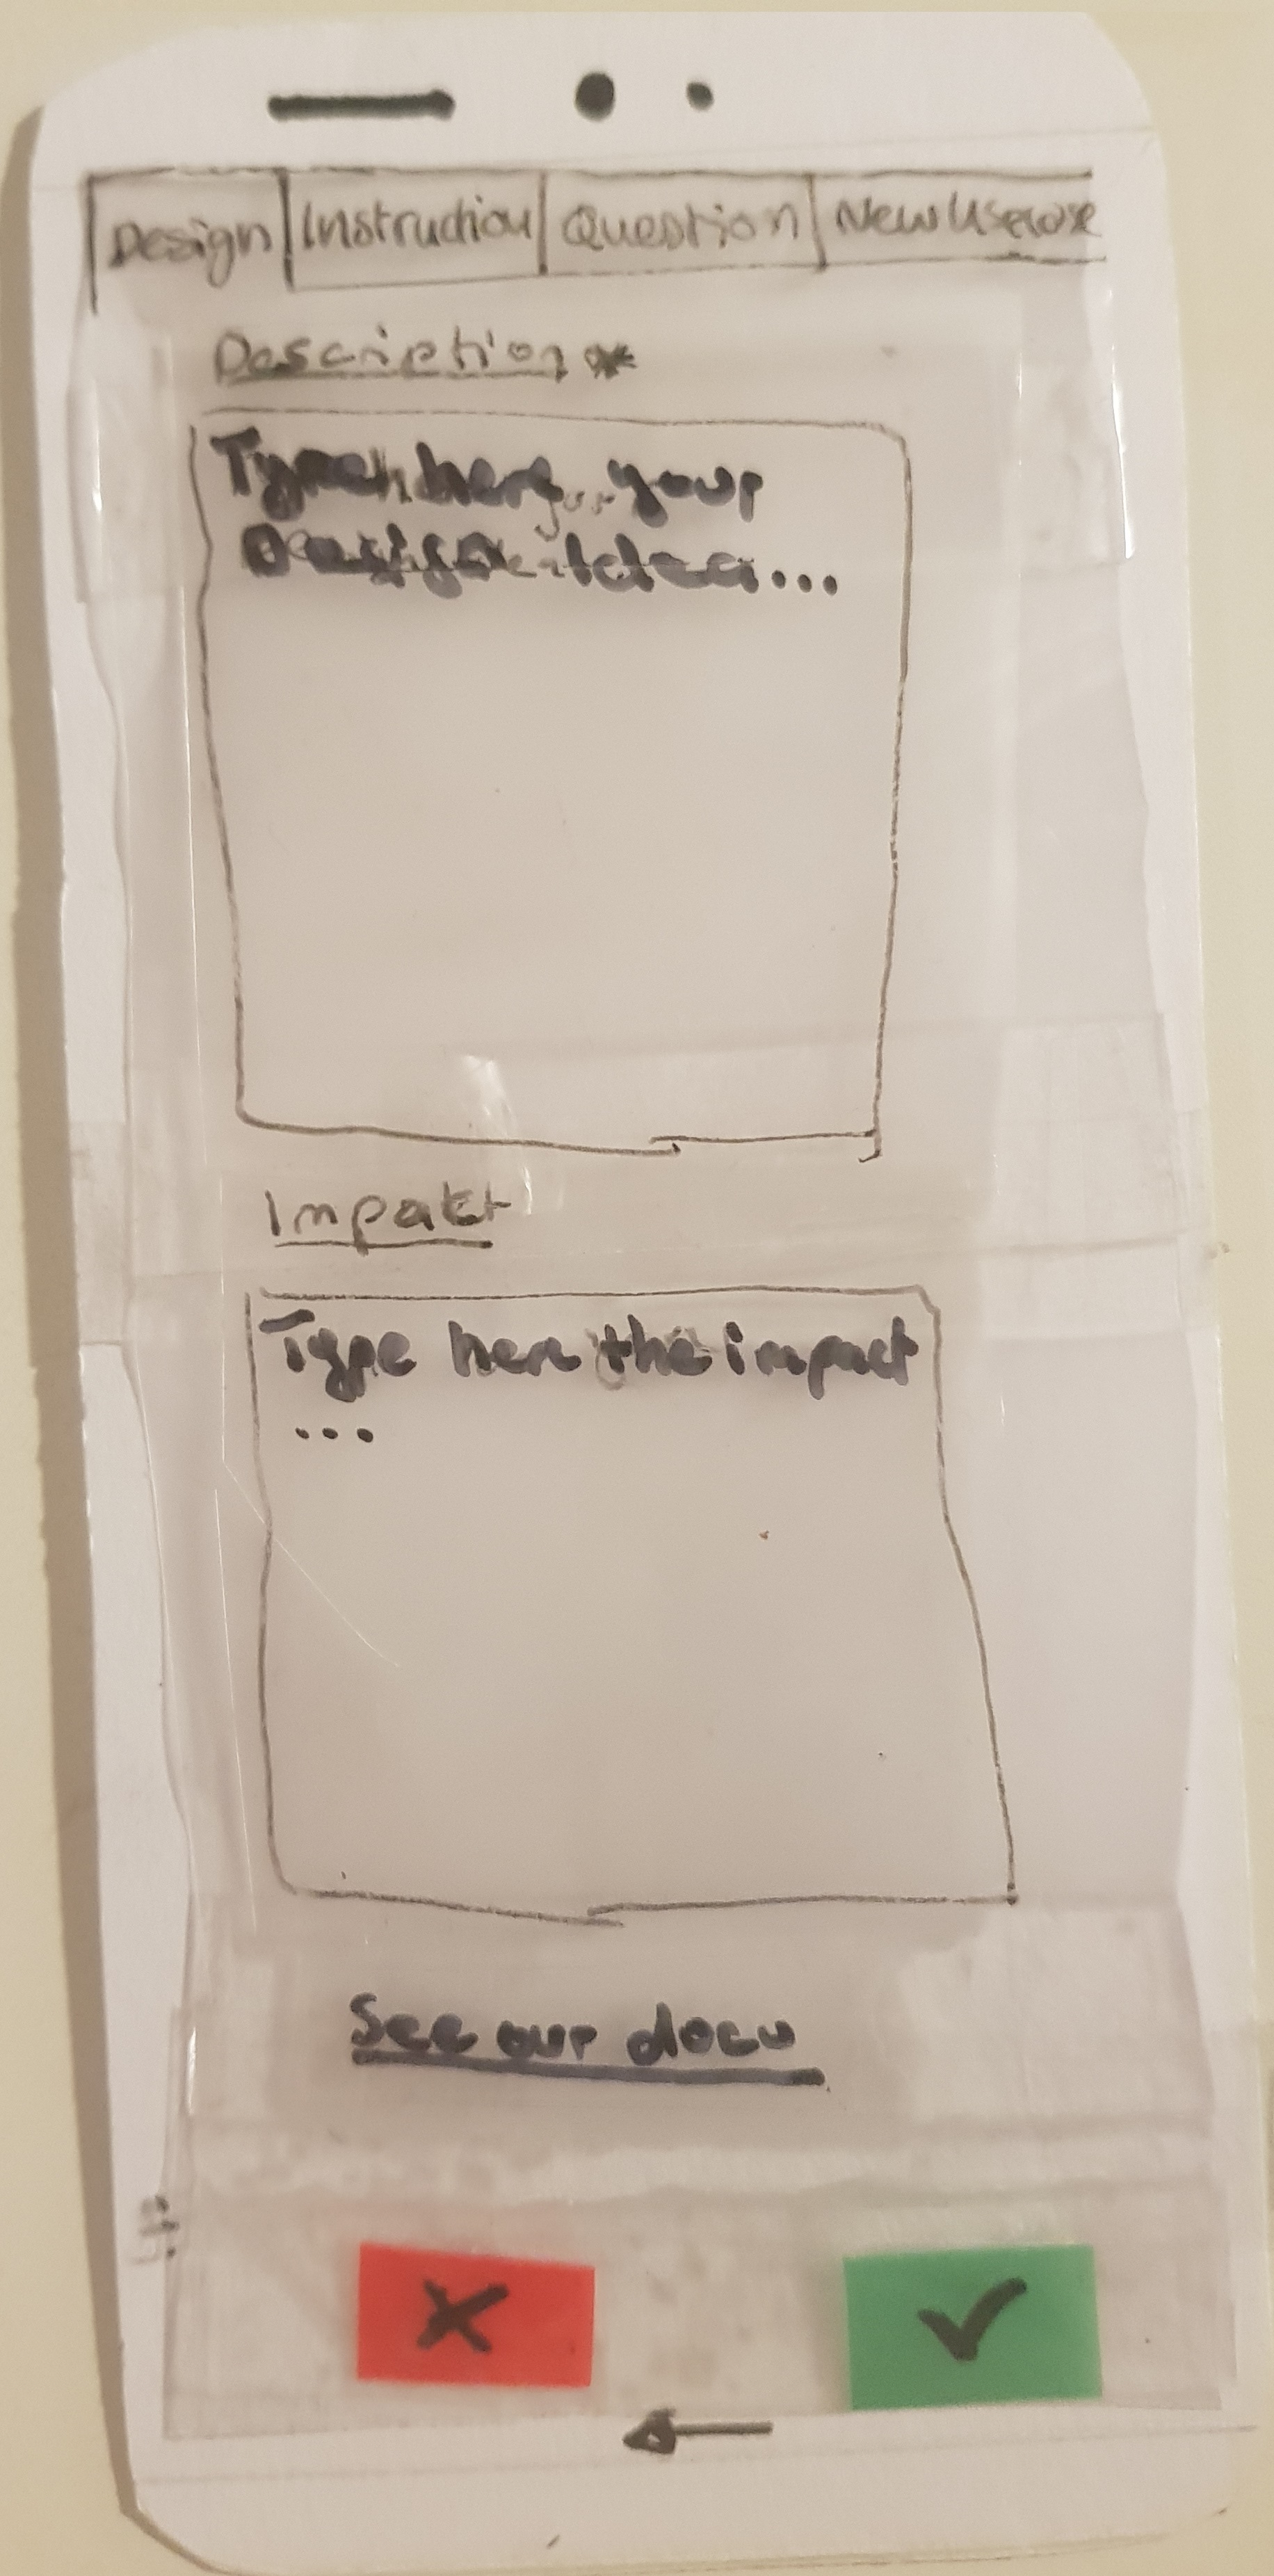
\includegraphics[width=.8\linewidth]{resources/conception/lowfi_form.jpg}
		\captionof{figure}{Papierprototyp - Eingabeformular für die \\Erstellung eines neuen Feedback.\\Quelle: Eigene Darstellung}
		\label{fig:test1}
	\end{minipage}%
	\begin{minipage}{.5\textwidth}
		\centering
		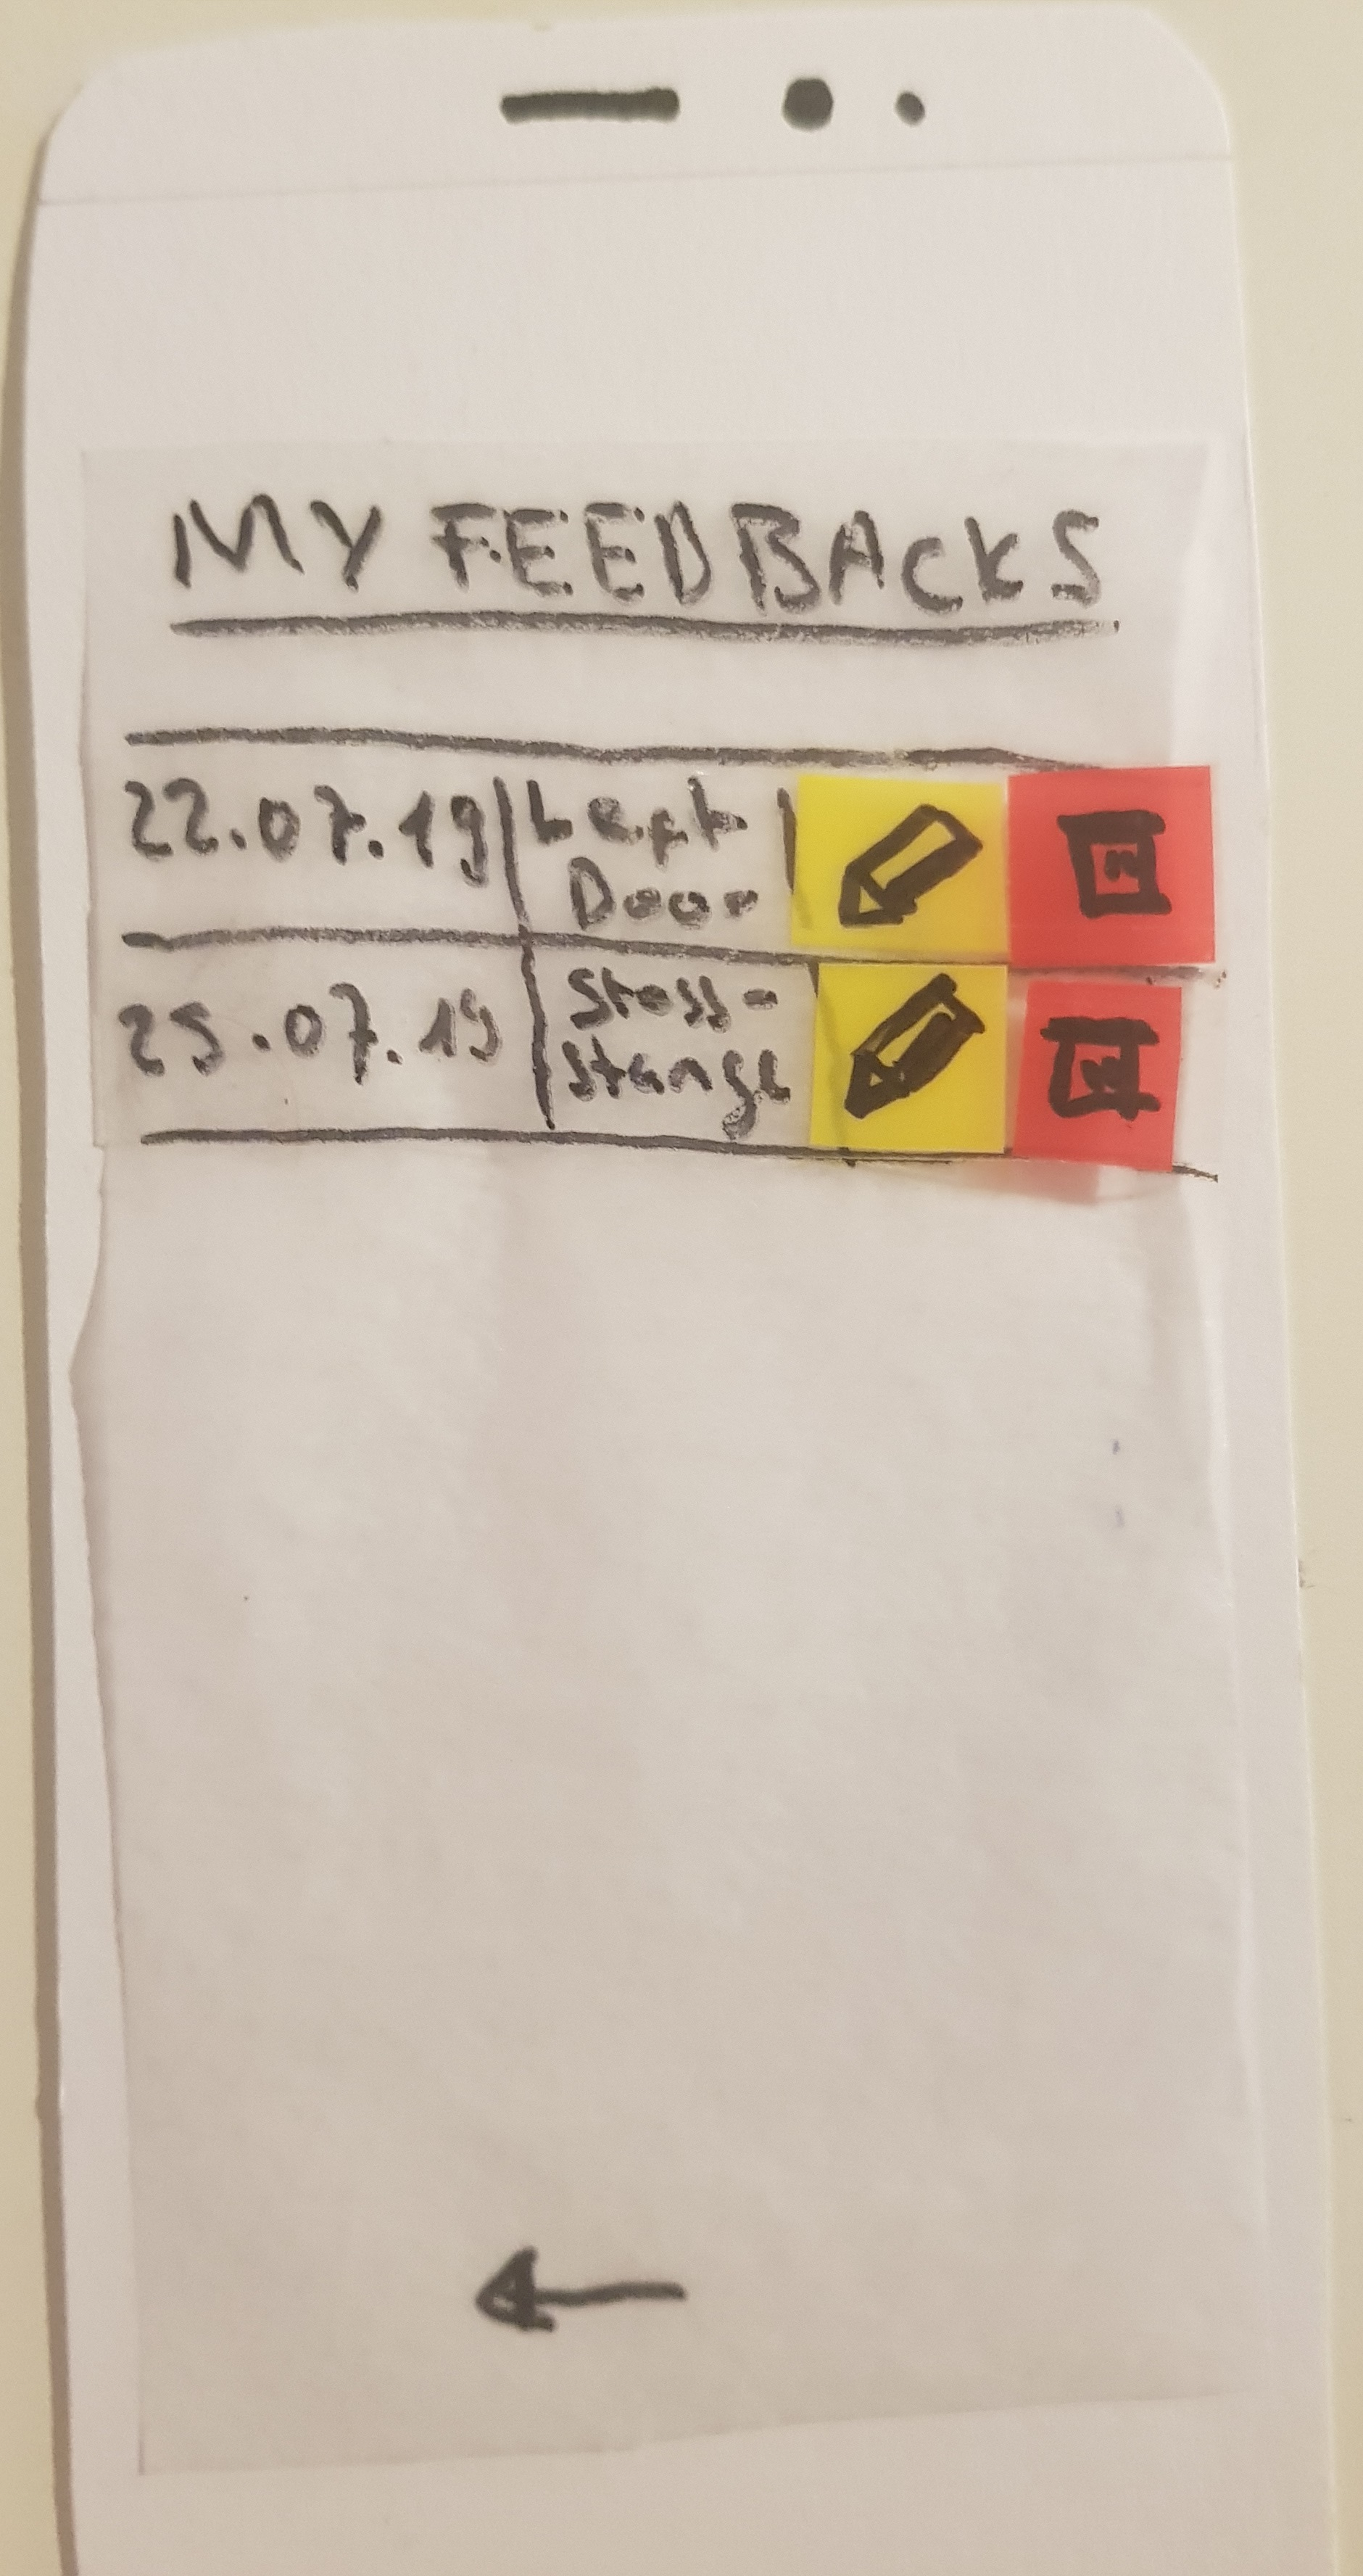
\includegraphics[width=.8\linewidth]{resources/conception/lowfi_list.jpg}
		\captionof{figure}{Papierprototyp - Listenansicht aller Feedback für die Bearbeitung bzw. Löschung.\\Quelle: Eigene Darstellung}
		\label{fig:pplist}
	\end{minipage}
\end{figure}

\subsection{Konzeptioneller Entwurf}




Entity Relationship Diagramm (ERM)


Klassendiagramm